\documentclass[a4paper,12pt,titlepage]{article}
\usepackage{amsmath}
\usepackage[serbian]{babel}
\usepackage{verbatim}
\usepackage{graphicx}
\usepackage{latexsym}
\usepackage[margin=1in]{geometry}
\usepackage{color}
\usepackage{listings}
\usepackage[utf8]{inputenc}
\usepackage[T1]{fontenc}
\usepackage{currvita}
\usepackage{hyperref} 
\usepackage{float}

\newtheorem{definicija}{Definicija}[section]
\newtheorem{teorema}{Teorema}[section]
\renewcommand{\contentsname}{Sadr\v zaj}
\renewcommand{\refname}{Literatura}
\renewcommand{\mod}[1]{$mod$ ${#1}$}

\title{\Huge {\textbf{Obrada slike korišćenjem Guided filtra}}}
\author{\textbf{Autor:} Predrag Nikolić \and \textbf{Mentor:} Dejan Rančić}
\date{\today}

\begin{document}
\begin{center}
\large Univerzitet u Nišu \\ Elektronski fakultet
\end{center}

\begin{minipage}{\textwidth}
   \maketitle
\end{minipage}
\thispagestyle{empty}
\newpage

\tableofcontents
\thispagestyle{empty}
\newpage

\pagenumbering{arabic} 
\section{Obrada slike}%%%%%%%%%%%%%%%%%%%%%%%%%%

\subsection{Uvod}%%%%%%%%%%%%%%%%%%%%%%%

Računarska grafika je oblast računarstva koja se bavi obradom, stvaranjem i modeliranjem slika i video materijala, korišćenjem kompjutera. 
Ovaj izraz se obično odnosi na kompjuterski generisane podatke u vidu slike, koji su kreirani uz pomoć specijalizovanog softvera ili hardvera.
Ova oblast se odnosi na sve iz sveta kompjutera što nije prikazano tekstom ili zvukom.
Naučnici su počeli da se bave problemima iz računarske grafike još 60-ih, a danas ona obuhvata mnoge podoblasti i prožima mnoge druge
obalsti kako računarskih tako i drugih nauka. Neke od tema kojima se bavi računarska grafika su dizajn korisničkog interfejsa, spite grafika, vektorska grafika, 3D modeling itd. Možemo da zaključimo da se proučavanje računarske grafike, kao deo računarskih nauka, bavi metodima
za digitalnu obradu i manipulaciju visuelnim sadržajem. Iako se računarska grafika obično odnosi na tro-dimenzionalnu kompjutersku grafiku
takođe obuhvata i dvo-dimenzionalnu grafiku i obradu slike. 

Obrada slike je proces kod kojeg se slika ili video (koji je ustvari niz slika) obrađuju da bi se dobila izmenjena slika (video) ili skup karakteristika
ili nekih bitnih parametara. Slike se u obradi tretiraju kao signali pa se za njihovu obradu koriste metode iz oblasti obrade signala i razne matematičke operacije. Ova obalst je takođe usko povezana sa kompjuterskom vizijom i naravno kompjuterskom grafikom. Kada se kaže obrada slika obično se misli na digitalne slike, ali je takođe moguća i obrada optičkih i analognih slika. 

Digitalna slika može da se definiše kao funkcija $f(x, y)$, gde su $x$ i $y$ koordinate ravni. $x$ i $y$ predstavljaju koordinate piksela na slici. Pikseli su elementi od kojih je sastavljena slika. Obično $x$ predstavlja vrednost u odnosu na širinu slike, a $y$ u odnosu na visinu slike. Rezolucija slike se obično obeležava kao širina puta visina, izraženo u pikselima. Vrednost funkcije $f$ je intenzitet boje piksela na poziciji $(x, y)$. Intenzitet može da bude izražen kao jedna vrednost, ako je u pitanju crno bela slika, ili preko tri vrednosti ako je slika u boji. Postoje različiti načini za predstavaljanje slike u boji (Npr. RGB, CMYK, HSV itd.). Vrednosti funkcije $f$ kao i $x$ i $y$ su diskretne, jer je reč o digitalnoj slici. 

Čulo vida je nasloženije čulo čoveka i ima možda i najveću ulogu u čovekovoj precepciji okoline. Međutim no ono nije savršeno. Za razliku od ljudskog vida koji je limitiran vidljivim elektromagnetnim spektrom, u računarstvu imamo mogućnost da predstavimo ceo spektar i da se bavimo talasnim dužinama koje naše oko ne može da vidi. Obrada slika je složena oblast i prožima mnoge druge oblasti. Ne postoje jasne granice između obrade slike i oblasti kompjuterskog vida. Sama obrada slike može da bude deo sistema veštačke inteligencije za prepoznavanje lica ili nešto slično. Za obradu slike možemo da je porces koji na ulazu uzima sliku,   
vrši obradu i na izlazu se nalazi ponovo slika, ali u toku obrade takođe računa atribute te slike. 

Potreba za korišćenjem digitalnih slika javila se još 1920-tih godina u novinarstvu. Tada je prvi put slika poslana prekookenaski putem analognog kabla. Naravno prvi problemi koji su se javili tada imali su veze sa kvalitetom slike. Prvi sistemi su mogli da prenose crno bele slike, do 15 nijansi sive. Prvi kompjuteri koji su bili dovoljno moći da izvršavaju neku značajniju obradu slika javili su se 60-ih godina. Neke od prvih primena bile su vezane za poboljšanje slika iz svemira. Zatim je obrada slika počela da se koristi u medicini i astronomiji 70-ih godina, a i dan danas je bitna u tim oblastima.

\begin{figure}[ht!]
\centering
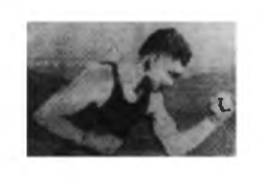
\includegraphics[width=75mm]{img/prvaPrenesenaSlika.png}
\caption{Digitalna slika koja je kreirana na osnovu kodirane trake 1921 godine}
\label{overflow}
\end{figure} 

U današnje vreme skoro da ne postoji oblast u kojoj se u nekoj meri ne koristi obrada slika. Jedna od najpoznatijih primena obrade slike je kreiranje i obrada rendgenskih slika (radiografija). Ona se najviše koristi u medicini ali postoje i druge primene. Primena postoji i za slike koje predstavljaju ultravioletnu boju. Ove slike se koriste u mikroskopiji. Postoje mnoge primene u svetu tehnologije kao što su izoštravanje slika, restauracija slika, prepoznavanje lica i objekata, prepoznavanje oblika. Takođe obrada slike se koristi u filmovima i medijima.  

Bitne komponente sistema za obradu slike su specijalizovan hardver za obradu slike, kao što su grafičke kartice, zatim kompjuter koji izvršava procese obrade slike i prikazuje rezultat. Takođe je bitan softver koji se koristi za obradu slike kao i komponente i metode za čuvanje velike količine podataka. Naravno možda i najbitniji komponenta je displej na kojem možemo da vidimo rezultat obrade slika.            

\subsection{Osnovni procesi u obradi digitalne slike}%%%%%%%%%%%%%%%%%%%%%%%

Neki od osnovnih procesa i primena u obradi digitalne slike su sledeći. \emph{Pribavljanje slike} \emph{(eng. Image acquisition)} se odnosi na to kako je slika nastala. Slika može da bude data u digitalnom obliku, a može da se zada i u analognom. Akvizicija slike uključuje predprocesiranje kao što je skaliranje i drugo. \emph{Poboljšanje slike} \emph{(eng. Image enhancement)} je najprostiji ali i najkorišćeniji postupak u obradi slika. Cilj ovog procesa je da se na slici izraze bitni aspekti radi izučavanja parametra neke slike. Primene su različite (npr. izoštravanje ivica radi uočavanja detalja). \emph{Restauracija slike (eng. Image restoration)} je oblast koja se bavi poboljšanjem izgleda slike. Razlika između restauracije i poboljšanja je u tome što se tehnike za restauraciju oslanjaju na matematičke i probabilističke modele degradacije slike, dok se poboljšanje zasniva na subjektivnom osećaju čoveka. \emph{Obrada slika u boji (eng. Color image processing)} je oblast koja se bavi obradom slike u boji i artifaktima koje slike u boji donose u odnosu na obradu crno belih slika. \emph{Kompresija (eng. Compression)} se bavi tehnikama za kompresiju slike, radi smanjenja veličine slika, što je od velikog značaja za prenos i čuvanje podataka. \emph{Morfološka obrada slike (eng. Morphological processing)} se bavi alatima za ekstrakciju komponenti slika koji su pogodni za određenu reprezentaciju podataka koje slika nosi. \emph{Segmentacija (eng. Segmentation)} se bavi podelom slike na koezistentne delove ili objekte. \emph{Reprezentacija i deskripcija (eng. Representation and description)} kao što samo ime kaže se bavi predstavljanjem slike kako na ulazu tako i na izlazu nekog procesa obrade slike. I na kraju \emph{Prepoznavanje (eng. Recognition)} je proces u kojem se objektima dodeljuju labele odnosno imena na osnovu deskriptora, koji se mogu dobiti na osnovu slike. Svi ovi procesi mogu da koriste bazu znanja u kojoj se čuvaju bitne činjenice za svaki od procesa prilikom obrade slika. Postupci i osobine koje se javljaju na određenoj slici mogu da se jave ponovo. pa je čuvanje podataka o obradi veoma bitno.

U ovom radu ćemo se fokusirati na pribavljanje slike i poboljšanje slike.

\subsection{Pribavljanje slike}%%%%%%%%%%%%%%%%%%%%%%%

Iako je oblast digitalne obrade slika izgrađena na onovu matematičkih i probabilističkih formaulacija, pribavljanje slike je proces koji je određen na osnovu ljudskog čula vida. Slika se u digitalnom svetu pribavlja nasličan nači na koji čovek vidi, ondnosno kreira sliku u mozgu. Ljudski preceptor za vid je oko. Prozirni prednji delovi oka lome zrake svetlosti projektujući umanjenu i obrnutu sliku na fotosenzitivnu mrežnjaču gde se u specijalizovanim nervnim ćelijama ovbavlja pretvaranje slike u električne nervne impulse. Zrak se prelama u očnom sočivu, a deo oka odgovoran za prikupljanje slike je žuta mrlja, gde su nervene ćelije najgušće raspoređene. Pored žute mrlje se nalazi početag vidnog živca koji je neosetljiv na svetlo, pa se njegova projektcija u vidom polju naziva crna mrlja. Nervni impulsi kreirani u ćelijama se prenosu u mozak koji spaja slike iz oba oka i okreće obrnutu sliku čime se stvara osećaj vida u ljudskom mozgu.

Svetslost koju mi opažamo ima određeni intenzitet i boju. Ljudsko oko je sposobno da vidi samo deo elektromagnetnog spektra. Ono može da detektuje svetlost koja se u sprektru nalazi izmedju ultavioletne i infracrvene boje. Posto se svetlost tretira kao talas, boju odnosno deo spektra određuje talasna dužina. Talasna dužina se predstavalja kao odnos brzine svetlosti i frekvencije svetla $\lambda = c / \nu$. Energija koju nosi talas se računa se kao $E = h \nu$, gde je $h$ Plankova konstanta, a $\nu$ je frekvencija talasa. Ljudsko oko vidi svetlost talasne dužine između $0.4 * 10^{-6}m$ i $0.7 * 10^{-6}m$.

\begin{figure}[ht!]
\centering
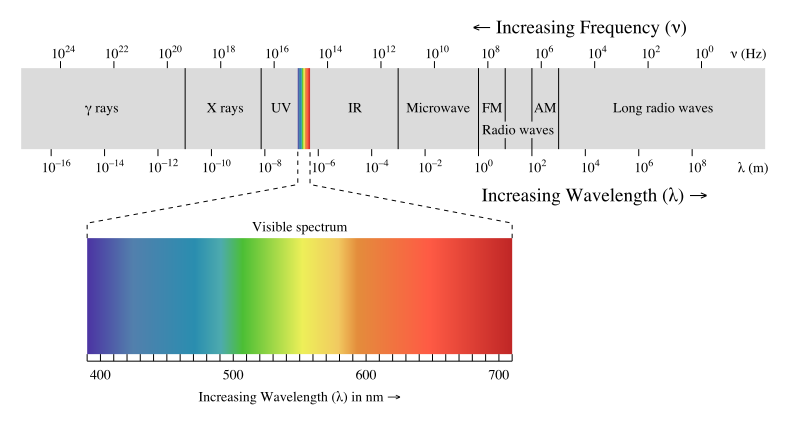
\includegraphics[width=120mm]{img/spektar.png}
\caption{Elektromagnetni spektar}
\label{overflow}
\end{figure} 

Slika se u digitalnom svetu generiše kao kombinacija osvetljenja prostora i reflektivne ili apsorbovane energije iz prostora scene za koju se pravi slika. Postoje raličiti tipovi senzora za akviziciju slika, ovde će biti opisan sistem sa senzorom u obliku 2-D niza (matrice). Senzor je sastavljen od elementata koji su raspoređeni u matrici. Svaki element je zadužen za prikupljanje svetlosti iz scene. U svakom elementu se beleži osveteljenje scene i tako se formira signal slike koji se kasnije dodatno obrađuje.

Pošto svetlost dolazi i kontinulanog prostora, vrednost signala koji nosi sliku će biti kontinualna. Da bi takav signal mogao da se obradi u računaru potrebno je da se taj signal digitalizuje. Digitalizaciju signala omogućuju semplovanje i kvantizacija. Semplovanje se odnosi na digitalizaciju koordinata piksela, odnosno određivanja mesta u prostoru. Kvantizacija se odonsi na digitalizaciju vrednosti amplitude signala. Pošto je slika skup određenog broja piksela od kojih svaki ima tačno određene koordinate u prostoru $(x, y)$, signal treba da se sampluje tako da svaki piksel bude popunjen jedinstvenom vrednošću. Vrednost amplitude signala je kontinualna, pa je kao takvu nemoguće sačuvati u računaru, zbog toga se uvodi kvantizacija gde se ta vrednost prevodi u diskretan prostor. Taj proces se naziva kvantizacija. Vrednost intenziteta piksela se obično predstavlja kao ceo broj izmedju 0 i 255. Postupak semplovanja i kvantizacije je bitan, jer od njega zavisi kvalitet i veličina podataka koje nosi signal slike. Ako je broj semplova ili kvantizacionih nivoa mali doći će do smanjenja kvaliteta slike, tj. slika neće biti verno prikazana. Međutim ako je broj  semplova ili kvantizacionih nivoa veliki broj podataka za čuvanje u memoriji će biti preveliki. U ovom postupku je bitno da se pronađe balans između ove dve stvari. U zavisnosti od potrebe će biti definisan broj semplova i kvantizacionih nivoa. Npr. nekada je bitnije da se sačuva što više slika, nego da slika bude precizna.  

Slika se u digitalnom svetu predstavlja kao $f(x, y)$, gde su $x$ i $y$ koordinate piksela na slici, a $f(x, y)$ je vrednost piksela u koordinatama $(x, y)$. 

\[
f(x, y)
=
\begin{bmatrix}
    f(0, 0) & f(0, 1) & f(0, 2) & \dots  & f(0, N - 1) \\
    f(1, 0) & f(0, 1) & f(1, 2) & \dots  & f(1, N - 1) \\
    \vdots & \vdots & \vdots & \ddots & \vdots \\
    f(M - 1, 0) & f(M - 1, 1) & f(M - 1, 2) & \dots  & f(M - 1, N - 1)
\end{bmatrix}
\]

gde su N i M respektivno širina i visina slike.

Broj piksela slike se računa kao $b = M * N$, ako je slika crno bela, odnosno intenzitet piksela je prikazan kao jedna vrednost. Ako je u pitanju slika u boji onda se vrednost funkcije $f(x, y)$ predsavalja kao vektor vrednosti $[i_{1} i_{2} \dots i_{k}]$, gde je $k$ broj kanala, ondosno broj boja kojima je prikazana slika (najčešće 3 ako je u pitanju slika u boji). Tada se broj piksela računa kao $b = M * N * k$.

\subsection{Bitne relacije između piksela}%%%%%%%%%%%%%%%%%%%%%%%

Piksel $p$ sa koordinatama $(x, y)$ ima horizontalne i vertikalne susede $(x + 1, y)$, $(x - 1, y)$, $(x, y + 1)$, $(x, y - 1)$. Ovo se naziva 4-suseda piksela. Ako se dodaju dijagonalni susedi $(x + 1, y + 1)$, $(x - 1, y - 1)$, $(x + 1, y - 1)$, $(x - 1, y + 1)$ onda dobijamo 8-suseda piksela. Povezanost je osobina koja se dosta koristi u obradi slike. Ako su pikseli susedi i ako imaju istu vrednost ili vrednost iz istog podopsega mogućih vrednosti piksela onda su oni povezani. Putanja niz piksela koji su povezani na slici.

Postoje nekoliko načina za računanje distance između piksela. Ako imamo piksele $p$, $q$ i $z$ sa koordinatama $(x, y)$, $(s, t)$ i $(v, w)$, $D$ će biti mera distance ako važi: \\

a) $D(p, q) >= 0 (D(p, q) = 0 akko p = q)$,

b) $D(p, q) = D(q, p)$,

c) $D(p, z) <= D(p, q) + D(q, z)$.\\

Euklidska distanca: 

\begin{center}
$D_{e}(p, q) = [ (x  - s)^{2} + (y - t)^{2} ]^{1/2}.$
\end{center} 

Euklidska distanca nije baš pogodna za sliku koja ima diskretne vrendosti pa se za distancu koriste:\\

$D_{4}$ distanca 4-suseda:

\begin{center}
$D_{4}(p, q) = |x - s| + |y + t|.$
\end{center} 

\[
\begin{bmatrix}
     &  & 2 &   &  \\
     & 2 & 1 & 2  &  \\
     2 & 1 & 0 & 1 & 2 \\
     & 2 & 1 & 2  &  \\
     &  & 2 &   &  \\
\end{bmatrix}
\].\\

$D_{8}$ distanca 8-suseda:

\begin{center}
$D_{8}(p, q) = max(|x - s|, |y + t|).$
\end{center} 

\[
\begin{bmatrix}
     2 & 2 & 2 & 2  & 2 \\
     2 & 1 & 1 & 1  & 2 \\
     2 & 1 & 0 & 1 & 2 \\
     2 & 1 & 1 & 1  & 2 \\
     2 & 2 & 2 & 2  & 2 \\
\end{bmatrix}
\].\\

\subsection{Osnovne operacije nad slikom}%%%%%%%%%%%%%%%%%%%%%%%

Glavni cilj poboljšanja slike je da se slika obradi na takav način, da krajnji rezultat zadovoljava odgovarajuću primenu. tehnika koja će da se koriti za obradu slike zavisi od konkretne primene i uslova koje rezultujuća slika treba da ispuni. Obrada slike se deli na dve kategorije: Obrada slike u prostornom domenu i obrada slike u frekvencijskom domenu. Prostorni domen se odonsi na ravan u kome se slika nalazi i metode koje izvršavaju operacije nad slikom u prostoru, dok se kod drugog tipa operacije izvršavaju nad slikom koja je predstavljena u obliku signala. U ovom radu će biti objašenjena obrada slike u prostornom domenu.

Kao što je navedeno obrada slike u prostronom domenu znači da se operacije izvršavaju nad pikselima. Ove procese možemo da označimo kao $g(x, y) = T[f(x, y)]$, gde je $f(x, y)$ početna slika, $g(x, y)$ obrađena slika, a $T$ je operator koji je definisan nad pikselima i njhovim susedima na slici $f$. Piksel $(x, y)$ i njegivi susedi prave pravougaonik, čiji je centar $(x, y)$, nad kojim se izvršava operacija $T$. Vrednost piksela $g(x, y)$ se računa kao vrednost piksela $f(x, y)$ i njegovih suseda, nad kojima se izvršavaju neke operacije. Ovaj proces se obično naziva konvolucija. Osnovni postupak obrade slike se izvršava tako što se za svaki piksel slike izvrši operacija nad tim pikselom i njegovim susedima i dobijena vrednost se dodeljuje tom pikselu. Postoje dva tipa dodele: dodela na mestu računanja kada se ista slika koristi za računanje i dodelu novih vrednosti i drugi tip dodele kod kojeg se dodela vrši na drugoj slici u piksel koji ima iste koordinate kao piksel kome se pristupa na slici koja se obrađuje.   

Ako vrednosti funkcija $f(x, y)$ i $g(x, y)$ predstavimo kao $r$ i $s$ respektivno, onda obradu slike možemo da predstavimo kao $s = T(r)$. U nastavku je da pregled nekih osnovnih transformacija nad slikom u prostornom domenu. Ove transformacije će biti predstavljene nad jednokanalnim slikama (slike čiji pikesli uzimaju samo jednu vrednost - nijansu sive boje). Što se tiče slika u boji postupak za ove transformacije je sličan. Transforamcije se ili vrše nad svakim kanalom nezavisno, ili se slika prevodi u sliku sa jednim kanalom (postoji više načina), pa se primenjuje određena transformacija.

Najosnovnija operacija koja može da se izvede nad slikom je negativ. Svaki piksel slike dobija inverznu vrednost u odnosu na svoju. Ako se vrednosti piksela kreću u granicama $[0, L - 1]$, rezultujuća vrednost se dobija kao $s = L - 1 - r$. Ova operacija se koristi na crno belim slikama koje su dominantno crne, a belom bojom su prikazani bitni podaci na slici, jer je lakse uočiti neke detalje.

\begin{figure}[ht!]
\centering
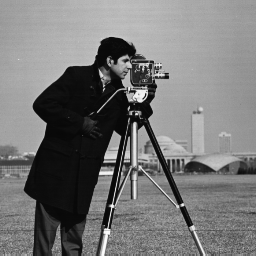
\includegraphics[width=60mm]{img/img.png}
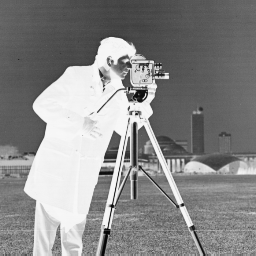
\includegraphics[width=60mm]{img/imgNegative.png}
\caption{1)slika 2)negativ}
\label{overflow}
\end{figure} 

Nad slikom može da se primeni logaritamska operacija. $s = c*\log{1+ r}$. Ova operacija se koristi za izračunavanje spektra slike, što može da bude korisno za operacije koje se izvršavaju u kompleksnom domenu. Takođe nad slikom možemo da primenimo i stepene funkcije $s  = c*r^{\nu}$ ili $s = c*(r + \epsilon)^{\nu}$, gde su $c$ i $\nu$ pozitivne konstante i $\epsilon$ je konstanta. Ove opercije se koriste za gama korekciju. Jedna od najpozantijih primena je u tv uređajima koji su koriste katodne cevi. Takođe se koristi i za magnetnu rezonancu kako bi se pojačale boje i time izrazili detalji. 

\begin{figure}[ht!]
\centering
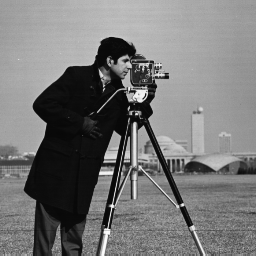
\includegraphics[width=60mm]{img/img.png}
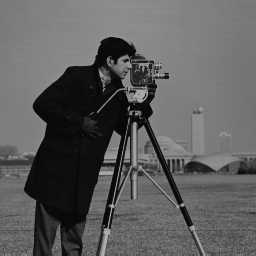
\includegraphics[width=60mm]{img/imgLog.png}
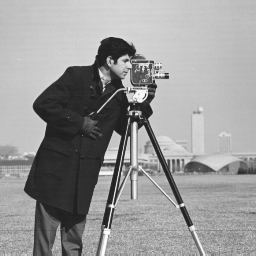
\includegraphics[width=60mm]{img/imgPow1.png}
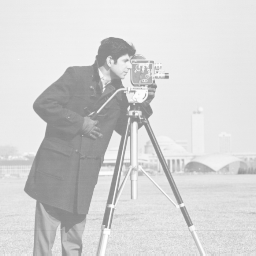
\includegraphics[width=60mm]{img/imgPow2.png}
\caption{1)slika 2)logaritamska transforamcija 3)stepena transforamcija $c = 1 \nu = 0.6$ 4)stepena transforamcija $c = 1 \nu = 0.3$}
\label{overflow}
\end{figure} 

Nasuprot predhodno navedena dva pristupa posoje i linearne transformacije. Nad slikom mogu da se izvode razne linearne funkcije. Neke od najkorićenijih su povećavaje kontrasta ili povećanje osvetljenja. Sve ove operacije imaju isti oblik $s = T(r)$, gde je T linearna transformacija, npr. menjanje osvetljenja slike može da se izrazi kao $s = r + c$ odnosno $s = r - c$, gde je $c$ konstanta u opsegu vrednosti koje uzimaju $s$ i $r$. 

Jedna od specifičnih obrada je obrada uz pomoć histograma. Histogram digitalne slike čiji pikseli uzimaju vrednosti iz $[0, L - 1]$ je diskretna funkcija $h(r_{k}) = n_{k}$, gde je $r_{k}$ k-ta vrednost u opsegu vrednosti koje uzimaju pikseli, a $n_{k}$ je broj piksela koji imaju tu vrednost. Obično se koristi noramlizovana f-ja $h(r_{k}) = n_{k}/n$, gde je n $max(n_{0}, n_{1}, ... , n_{L - 1})$, pa će sve vrednosti funkcije $h$ biti u opsegu $[0, 1]$. Histogrami mogu da se prikažu i grafički i oni nam ukazuju na to koje su nijanse zastupljene i kojoj meri na slici.  

\begin{figure}[ht!]
\centering
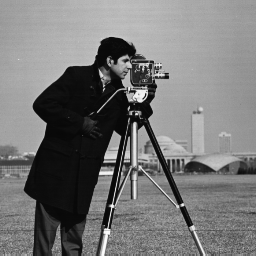
\includegraphics[width=60mm]{img/img.png}
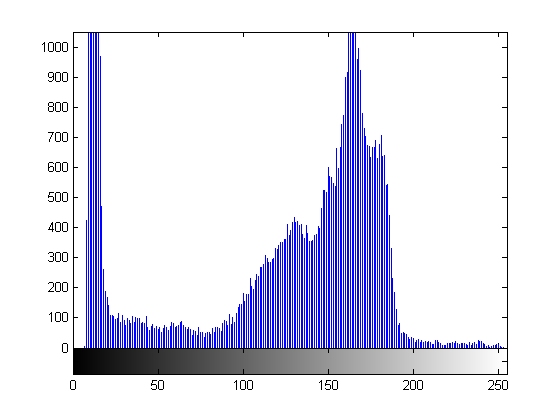
\includegraphics[width=60mm]{img/histImg.png}
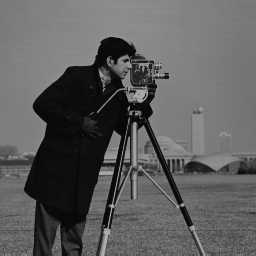
\includegraphics[width=60mm]{img/imgLog.png}
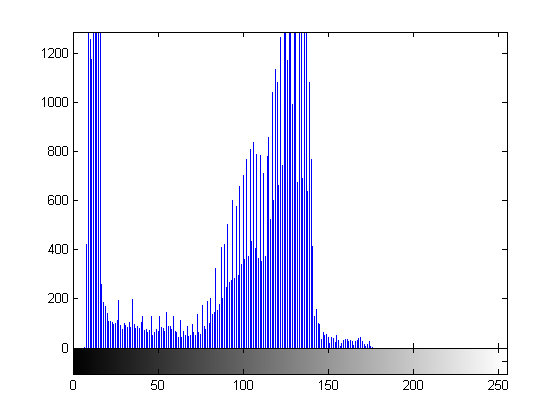
\includegraphics[width=60mm]{img/histImgLog.png}
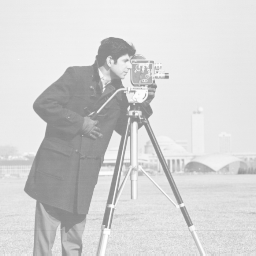
\includegraphics[width=60mm]{img/imgPow2.png}
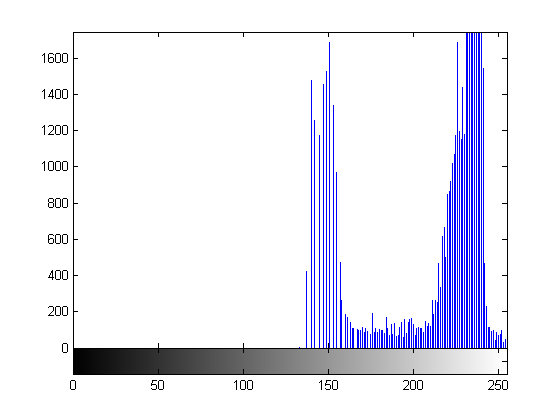
\includegraphics[width=60mm]{img/histImgPow2.png}
\caption{levo: slika desno: njen histogram}
\label{overflow}
\end{figure} 

Obrada slike uz pomoć histograma se vrši tako što se izračuna histogram slike, nad njim se izvrši transformacija, a zatim pikseli na slici dobiju odgovarajuće vrednosti na osnovu transformisanog histograma. Nad histogramom mogu da se izvrše razne operacije u cilju pobolšanja slike.   
Jedna od operacija koja može da se izvrši uz pomoć histograma je histogramsko izjednačavanje. Cilj ovog postupka je da napravi uniformi histogram, tj. da na slici sve nijanse budu jednako zastupljene. Ovo je korisna transformacija ako je na slici dominiraju iste nijanse. Ako na slici dominirju određeni broj nijansi slika može da bude nejasna, izjednačavanjem odnosno uniformisanjem histograma dobijamo sliku koja ima zastupljene sve nijanse, što će dovesti do vizuelnog poboljšanja slike. Ovde ne zalazimo detaljno u aspekte obrade slike pomoću histograma, jer ona nije od važnosti za ovaj rad.

\begin{figure}[ht!]
\centering
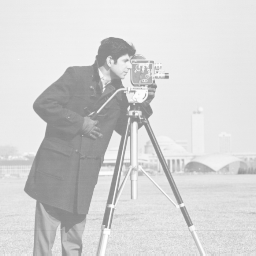
\includegraphics[width=60mm]{img/imgPow2.png}
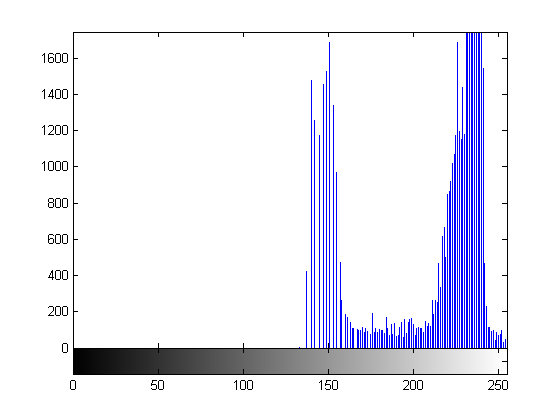
\includegraphics[width=60mm]{img/histImgPow2.png}
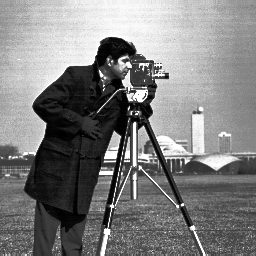
\includegraphics[width=60mm]{img/histEq.png}
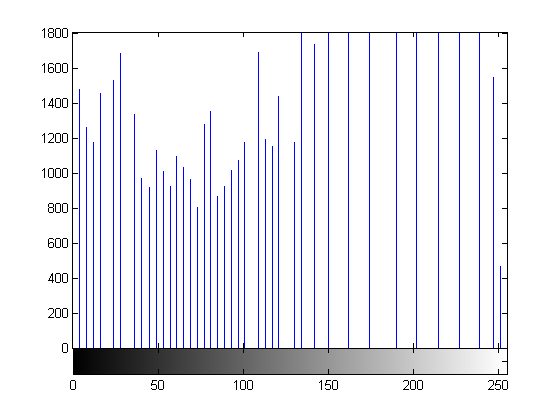
\includegraphics[width=60mm]{img/histEqhist.png}
\caption{1)slika 2)histogram 3)slika i 4)histogram nakon histogramskog izjednačavanja}
\label{overflow}
\end{figure}

Nad slikama možemo da primenimo i aritmetičke i logičke operacije. Logičke operacije AND, OR i NOT mogu da se primene nad slikama. AND operacija može da se koristi da bi se sa slike izvukao određeni region od značaja. Region može da se izvuče tako što će se primeniti AND operacija nad slikom i maskom. Maska je slika koja sadrži informaciju koji deo slike želimo da ostavimo. Maska se formira tako što se na mestima koje želimo da sadržimo stavaljmo maksimalnu vrednost koju uzimaju pikseli. Ako je opseg nijansi $[0, 1]$ onda je to 1, na svim ostalim mestima stavlja se 0. Rezultat ove operacije biće deo slike određen maskom. Na isti način se primenjuju i OR i NOT operacije. Logičke operacije su značajne za morfološku obradu slike koja je spomenuta kao jedna od oblasti kojima se bavi obrada slike. 

Nad slikama se često pirmenjuje operacija oduzimanja. Ako želimo da vidimo da li se dve slike razlikuju možemo da ih oduzmemo jednu od druge, što će da nam ukaze na razlike, jer će mesta gde su pikseli isti biti 0 tj crna a mesta gde ima ralike će biti predstavljena određenom nijansom. U ovu svrhu može da se koristi i deljenje. Sabiranje i množenje može da se koristi u svrhu dodavanja detalja na slici. 

\section{Osnovni tipovi filtara}%%%%%%%%%%%%%%%%%%%%%%%

\subsection{Osnovni pojmovi}%%%%%%%%%%%%%%%%%%%%%%%

Kao što je ranije spomenuto prilikom obrade slike operacije se izvršavaju nad pikselom i njegovim susedima sa jedne strane i ogovarajućom podslikom sa druge. Ta pod slika nosi informacije o koje se koriste za filtriranje slike. Ta podslika (odnosno pravougaonih piksela) se naziva kernel ili prozor. Koncept filtriranja slike je uzet iz matematike ondnosno analize i matematički predstavljen taj proces je ustvari konvolucija $f * w$ gde je $f$ predstavlja sliku koja se filtrira, $w$ predstavlja kernel za filtriranje. Za svaki piksel slike koja se filtrira računa se nova vrednost uz pomoć kernela $w$ i odgovarajućeg piksela i njegovih suseda, iz slike. Ako imamo kernel oblika $3 x 3$ iračunavanje vrednosti piksela $(x, y)$ izgleda ovako

\begin{center}
$R = w(-1, -1)f(x - 1, y - 1) + w(-1, 0)f(x - 1, y) + \dots + w(0, 0)f(x, y) + \dots + w(1, 0)f(x + 1, y) + w(1, 1)f(x + 1, y + 1)$.
\end{center}

\[
R
=
\begin{bmatrix}
     f(x - 1, y - 1) & f(x - 1, y) & f(x - 1, y + 1) \\
     f(x, y - 1) & f(x , y) & f(x, y + 1) \\
     f(x + 1, y - 1) & f(x + 1, y) & f(x + 1, y + 1) \\
\end{bmatrix}
.*
\begin{bmatrix}
     w(- 1, - 1) & w(- 1, 0) & w(- 1, 1) \\
     w(-0, - 1) & w(0, 0) & w(0, 1) \\
     w(1, - 1) & w(1, 0) & w(1, 1) \\
\end{bmatrix}
\].

Koeficijet kernela $w(0, 0)$ odgovara pikselu $f(x, y)$, što ukazuje na to da je maska centrirana oko piksela $(x, y)$. Obzirom da kernel mora da bude centriran oko jednog piksela, za kernel dimenzije $m x n$, važi da je $m = 2a + 1$ i $n = 2b + 1$, gde su $a$ i $b$ pozitivni celi brojevi. Najmanji kernel koji ima smisla je $3 x 3$ , a trivijalni slučaj predstavlja kernel $1 x 1$, koji se primenjuje samo kod osnovnih operacija. Generalno filtriranje slike $f$ dimenzija $M x N$, korišćenjem kernela $w$ veličine $m x n$ izrazom:

\begin{center}
$g(x, y)  = \sum_{s = -a}^{a} \sum_{t = -b}^{b} w(s, t) f(x + s, y + t)$,\\
\end{center}

gde je $a = (m - 1) / 2, b = (n - 1) / 2$. Da bi se filtrirala cela slika potrebno je da se i zračuna vrednost $g(x, y)$ za svako $x \epsilon [0, M - 1]$ i za svako $y \epsilon [0, N - 1]$. 

Matrica kernela može da se obelži i ovako za primer kernela $3 x 3$:

\[
R
=
\begin{bmatrix}
     z_{1} & z_{2} & z_{3} \\
     z_{4} & z_{5} & z_{6} \\
     z_{7} & z_{8} & z_{9} \\
\end{bmatrix}
.*
\begin{bmatrix}
     w_{1} & w_{2} & w_{3} \\
     w_{4} & w_{5} & w_{6} \\
     w_{7} & w_{8} & w_{9} \\
\end{bmatrix}
\].

\begin{center}
$R = w_{1}z_{1} + w_{2}z_{2} + \dots + w_{mn}f_{mn} = \sum_{i = 1}^{mn} w_{i}z_{i}$.\\
\end{center}

$w_{i}$ predstavlja vrednosti kernela, $z_{i}$ predstavlja vrednosti odgovarajućih piksela slike, a $m$ i $n$ predstavljaju dimenzije kernela.

Možemo da kažemo da se filtriranje obavlja tako što kernel prolazi kroz celu sliku. Ovaj pristup se koristi kako za linearne tako i za nelinerane filtre. Bitno je obratiti pažnju na piksele slike koji se nalaze uz ivicu slike. Ti pikseli nemaju sve susede pa oni moraju na neki načina da se dodele. To može da se reši na više različitih načina, a neki od uobičajnih su postavljanje vredosti tih suseda na 0 ili neku drugu konstantu ili uzimanje vrednosti simetričnih piksela u odnosu na piksel za koji se vrši konvolucija. 

Dva osnovna tipa filtera su filteri za uklanjanje šuma i zamućivanje slike koji se nazivaju smoothing filteri i filteri za izoštravanje slike, odnosno filteri za određivanje ivica ivica koji se nazivaju sharpening filteri. Pošto ne postoji tačan prevod za ove nazive dalje u radu se koriste imena smoothing i sharpening.

\subsection{Smoothing filtri(filtri za uklanjanje šuma)}%%%%%%%%%%%%%%%%%%%%%%%

Ovaj tip filtra se koristi za takozvano zamućivanje \emph{(eng. blurring)} i za redukciju šuma. Blurring se koristi za uklanjanje malih detalja sa slike, u procesu ekstrakcije objekata sa slike. Takođe može da se koristi za popunjavanje prekida u linijama na slici, koje mogu da se jave zbog šuma na slici. Rezultat ovog filtra je u suštini srednja vrednost piksela koji su sadržani u okolini kernela koji se koristi za filtriranje. Zbog toga se ovi filtri nazivaju i filteri srednje vrednosti \emph{(eng. averaging filters)}. 

Ideja ovog filtriranja je da se vrednost konkretnog piksela zameni sa srednjom vrednošću piksela iz njegove okoline, koji su definisani kernelom. Rezultat ovog filtra biće slika koja ima ublažene prelaze između vrednosti susednih piksela. Dva susedna piksela koja se dosta razilkuju biće sličnija po vrednosti. Pošto se pikseli, koji predstavaljaju šum, dosta razlikuju po vrednost od susednih piksela, na ovaj način će se oni uklopiti u okolinu. Loša strana ovakvog filtriranja se ogleda u tome što će mesta koja predstavalju ivice ili linije na slici početi da gube oštrinu. Naime na mestima na kojima se nalaze ivice imamo veliku razliku u susednim pikselima, pa će primenom ovog filtra ta ralika postati manja što će dovesti do gubljenja oštrine tih ivica.  

\[
1/9
*
\begin{bmatrix}
     1 & 1 & 1 \\
     1 & 1 & 1 \\
     1 & 1 & 1 \\
\end{bmatrix}
1/16
*
\begin{bmatrix}
     1 & 2 & 1 \\
     2 & 4 & 2 \\
     1 & 2 & 1 \\
\end{bmatrix}
\].     

Ovo su tipični primeri smoothing filtra dimenzija $3 x 3$. Levo je najprostiji primer ovog tipa filtara. Primenom ovog kernela svaki piksel će dobiti kao rezultat prosečnu vrednost susednih piksela koji odgovaraju obliku ovog kernela. Koeficijent $1/9$ služi da bi se dobila strdnja vrednost. Rezultat koji će biti upisan u piksel je $R = 1/9 \sum_{i = 1}^{9} z+{i}$. Kao što vidimo na primeru kernela sa desne strane, ne moraju svi susedni pikseli da učestvuju podjednako u sumi. Na ovom primeru vidimo da pikseli različito učestvuju u sumi sa različitim koeficijentima koji su definisani u kernelu. Te vrednosti se nazivaju težine. Vidimo da se i koeficijent koji stoi uz kernel razlikuje u odnosu na primer levo. On je $1/16$, jer je suma brojeva iz kernela $16$. U većini slučajeva se ovaj koeficijent određuje na ovaj način. Na ovom primeru vidimo da se prilikom filtriranja daje prednost samom pikselu, jer uz njega stoji najveći koeficijent 4, zatim se daje prednost horizontalnim i vertikalnim susedima, oni imaju koeficijente 2 i tek na kraju su dijagonalni susedi sa koeficijentom 1. Ovi koeficijenti u nekim slučajevima mogu da budu i 0.

\begin{figure}[ht!]
\centering
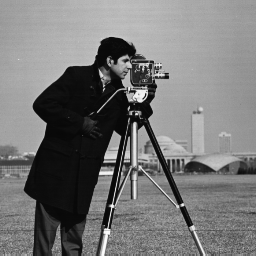
\includegraphics[width=60mm]{img/img.png}
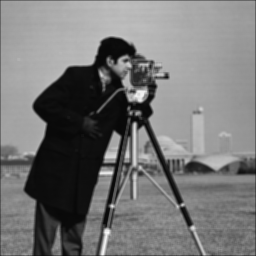
\includegraphics[width=60mm]{img/imgAvg3.png}
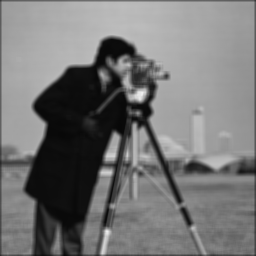
\includegraphics[width=60mm]{img/imgAvg5.png}
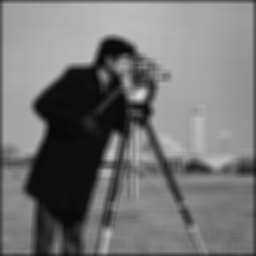
\includegraphics[width=60mm]{img/imgAvg9.png}
\caption{1)slika 2)slika filtrirana kernelom 3x3 3)5x5 i 4)9x9}
\label{overflow}
\end{figure}


Naravno ova priča važi i za filtre koji koriste kernel bilo koje dimenzije $m x n$ ($m$ i $n$ su neparni). Ako imamo kernel ovih dimenzija opšta formula za izračunavanje vrednosti rezultujećeg piksela igledaće ovako: 

\begin{center}
$g(x, y) = \dfrac{\sum_{s = -a}^{a} \sum_{s = -b}^{b} w(s, t)f(x + s, y + t)}{\sum_{s = -a}^{a} \sum_{s = -b}^{b} w(s, t)}$,  \\
\end{center}

gde su $g$ i $f$ ulazna i rezultujuća slika, $(x, y)$ koordinate piksela za koji se trenutno računa vrednost, $a = (m - 1) / 2$, $b = (n - 1) / 2$, $w$ težine u kernelu. Da bi cela slika bila filtrirana ova funkcija treba da se izvrši za svako $x \epsilon [0, M - 1]$ i za svako $y \epsilon [0, N - 1]$. 

Kao što je navedeno kerneli ovih filtra su proizvoljnih veličina. Za ovaj tip filtra se obično koriste $n x n$ kerneli, jer oni uzimaju simetrične piksele i najbolje određuju koliko se neki piksel razliku je u odnosu na njegovu okolinu. Težine definisane u kernelu određuju kojim susedima se daje prednost pilikom računanja srednje vrednosti. Npr. ako neka slika ima dosta vertikalnih ivica, težina koja će stojati uz piksele, koji su vertikalni susedni u odnosu na piksel za koji se računa vrednost, može da bude 0 da bi se izbeglo gubljenje oštrine. Veličina dimenzija kernela utiče na to koliko se brojčano uzima suseda, što će na krajnjem rezultatu uticati na to u kojoj je količini slika zamućena. Što su veće dimenzije kernela, veća će biti zamućenost na slici. Pošto je svaka slika drugačija, ona će zahtevati određenu kombinaciu težina i dimenzije kernela. Ovo se obično određuje probom različitih kernela da bi se utvrdilo koji je najbolji za konkretnu sliku. 

Kao što je spomenuto ranije jedna od primena ovog tipa filtara je predprocesiranje slike zarad uklanjanja sitnih detalja koji nisu od važnosti. Ovo se primenjuje prilikom ekstrakcije objekata sa slike mogu da se u određenoj meri ukolne sitni objekti da bi se olakšala ekstrakcija bitnih objekata. Veličina kernela će odrediti koja koji će objekti biti uklonjeni sa slike. Ako se koristi kernel veličine $3 x 3$ sa slike će biti uklonjene samo tačke veličine 1 piksela. Povećanjem dimenzija kernela biće uklonjene i veći objekti. Odabir veličine kernela zavisiće od toga šta želimo da odstranimo sa slike.

\begin{figure}[ht!]
\centering
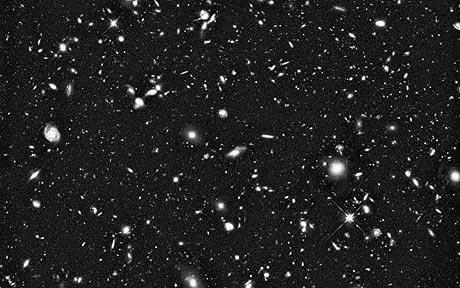
\includegraphics[width=60mm]{img/tel.jpg}
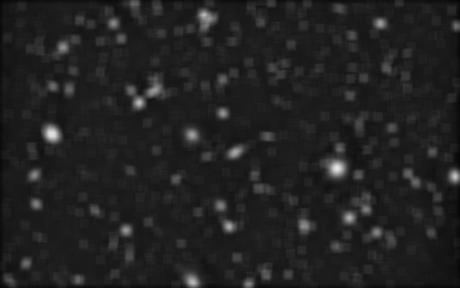
\includegraphics[width=60mm]{img/telAvg.jpg}
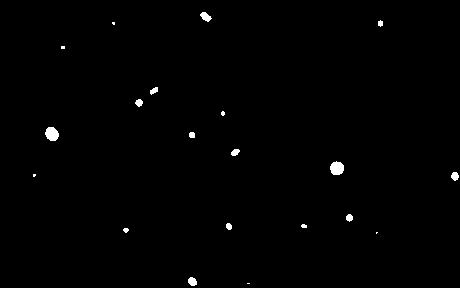
\includegraphics[width=60mm]{img/telTh.jpg}
\caption{1)slika 2)slika filtrirana kernelom 9x9 3)slika pretvorena u binarnu sliku(samo crna i bela)}
\label{overflow}
\end{figure}

Pored navedenih linearnih filtra postoje i nelinearni filtri bazirani na sortiranju vrednosti piksela koji se nalaze u oblasti koja je obuhvaćena filtriranjem, odnosno određena kernelom. Njapoznatiji primer je medina filter. Vrednosti u kernelu ondnosno težine koje se koriste u ovom filtru su 1. Pikseli iz željene oblasti se sortiraju i bira se vrednost koja se u tako sortiranom nizu piksela nalazi na sredini. Ona se dodeljuje pikselu koji se trenutno obrađuje. Ako koristimo kernel veličine $3 x 3$ nakon što sortiramo njihove vrednosti za rezultat ćemo odabrati 5-ti piksel po veličini (nije bitno da li se sortiraju rastuće ili opadajuće). Dakle vrednost piksela se zamenjuje sa pikselom iz njegove okoline koji ima statistički srednju vrednost. Median filter je efikasan za uklanjanje slučajnog šuma, a posebno je efikasan za uklanjanje šuma koji se naziva biber i so, a specifičan je po tome što se iskazuje preko crnih i belih tačaka, koje su minimalna i maksimalna vrednost koju piksel može da uzme, pa se zbog toga naziva i impulsni šum. Za ove primene medina filter je efikasniji od predhodno navedenih filtra, jer bira vrednost koja se najviše javlja u okolini određenog piksela.

\begin{figure}[ht!]
\centering
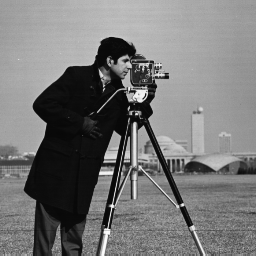
\includegraphics[width=60mm]{img/img.png}
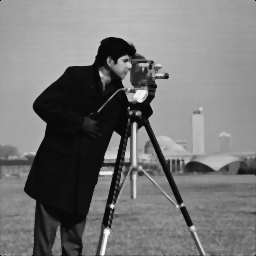
\includegraphics[width=60mm]{img/imgMed.png}
\caption{1)slika 2)slika filtrirana median filterom}
\label{overflow}
\end{figure}

\subsection{Sharpening filtri(filtri za određivanje ivica)}%%%%%%%%%%%%%%%%%%%%%%%

Glavni cilj ovog tipa filtara je da na slici obeleže fine detalje, kao što su linije i prelazi, ili da poboljša izgled tih detalja, koji mogu biti mutni ili da imaju grešku, koja je posledica određenog metoda pribavljanja slike. Primena ovih filtara je veoma široka i varira od elektronskog štampanja preko medicine do industrijske inspekcije i autonomnih vojnih i sistema nadzora. 

Filteri opisani u predhodnom poglavlju koriste sume i srednje vrednosti da bi filtrirali sliku. Ovaj proces je analogan integraciji, pa možemo da zaključimo da sharpening filtri, koji imaju suprotni cilj u odnosu na smooothing filtre, koriste diferenciranje da bi postigli željeni rezultat. Delovanje funkcije izvoda je porporcionalno stepenu nepovezanosti slike u tački, gde je izvod primenjen. Diferenciranje slika će naglasiti ivice i prelaze, kao i šum i sve delove gde se vrednosti piksela naglo menjaju (prelaz izmedju dve boje na slici koje se dosta razlikuju u nijansi npr crna i bela).

Da bi objasnili uticaj izvoda na sliku, objsnićemo osnovne koncepte preko jedno dimenzionalnih izvoda. Izvod diskretne funkcije se definiše kao razlika između dva uzastopna elementa. Postoji više načina za definisanje izvoda nad slikom, ali svi oni zahtevaju da funkcija izvoda ispunjava sledeće: 1) jednaka je nuli u ravnim segmentima (segmenti koji imaju konstantnu vrednost); 2) različita je od nule u segmentima gde postoji nagla ili konstantna promena; 3) različita je od nule duž segmenata gde se javlja konstantna promena; Slično i za funkciju drugog izvoda važi da je: 1)  jednaka je nuli u ravnim segmentima; 2) različita je od nule na mestima gde se završava nagla ili konstantna promena; 3) jednaka je nuli duž segmenata gde se javlja konstantna promena; S obzirom da pikseli slike uzimaju diskretne vrenosti vrednost izvoda se kreće u granicama tih vrednosti. Definicija jednodimenzionalnog izvoda je: 

\begin{center}
$\dfrac{\delta f}{\delta x} = f(x + 1) - f(x)$, parcijalni izvod po x osi.\\
\emph{} \\
$\dfrac{\delta f}{\delta y} = f(y + 1) - f(y)$, parcijalni izvod po y osi.\\
\end{center}

Slično se za drugi izvod definiše:

\begin{center}
$\dfrac{\delta^2 f}{\delta x} = f(x + 1) + f(x - 1) - 2f(x)$, drugi parcijalni izvod po x osi.\\
\emph{} \\
$\dfrac{\delta^2 f}{\delta y} = f(y + 1) + f(y - 1) - 2f(y)$, drugi parcijalni izvod po y osi.\\
\end{center}

\begin{figure}[ht!]
\centering
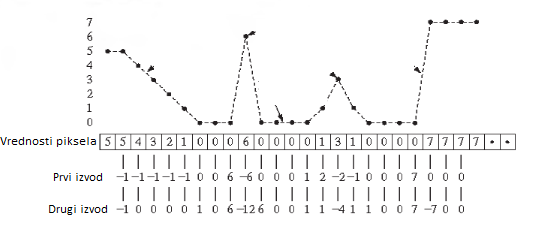
\includegraphics[width=120mm]{img/izvod.png}
\caption{Prvi i drugi izvod nad nizom piksela}
\label{overflow}
\end{figure}

Ako pogledamo sliku 10 možemo da uočimo da je prvi izvod različit od nule u segmentu gde je pad konstantan (svi susedi se razlikuju za 1), dok je drugi izvod različit od nule na početku i kraju tog segmenta. Pošto se ivice na slici iskazuju u ovom tranzicijom, možemo da zaključimo da će prvi izvod da proizvede debele ivice, dok će drugi izvod proizvesti tanke ivice. Npr. ako imamo belu liniju na crnoj pozadini, koja ima određenu debljinu, prvi izvod će izdvojiti celu liniju. Drugi izvod će ,sa druge strane, izdvojiti dve finije linije koje ukazuju na prelaz sa crne na belu boju i sa bele na crnu liniju. Ako pogledamo deo na kome imamo izolovani skok u vrednosti piksela, možemo da primetimo da je drugi izvod izraženiji nego prvi. Ovo je normalno jer je drugi izvod bolji u pronalaženju oštrih promena. Na osnovu ovoga možemo da očekujemo da će drugi izvod bolje da pronalazi finije detalje i šum. Ako je u pitanju manja promena prvi i drugi izvod će se ponašati slično. Na osnovu svega rečenog možemo da zaključimo da primenom prvog izvoda dobijamo debele lvice, dok primenom drugog izvoda dobijamo finije linije i izolirane tačke. Prvi izvod nam ukazuje na mesta gde je promena konstantna. Drugi izvod nam ukazuje na mesta gde je promena velika i izolovana. Ugalvnom se drugi izvod više koriti u konkrentim primenama zbog toga što naglašava finije detalje. Zbog toga ćemo se ovde fokusirati na filtre koje koriste drugi izvod. Bitno je naglasiti da se filteri koji koriste prvi izvod analogno koriste i imaju iste osobine kada se koriste.

Nad slikom se primenjuju dvo-dimenzionalni izvodi, jer slika ima dve dimenzije. Na osnovu ovoga se formiraju kerneli koji se koriste u primeni ovih filtara. Nas interesuju izotropski filteri, tj. filteri koji su invarijantni u odnosu na pravac promena, koje se javljaju na slici. Drugim rečima ovi filteri su nezavisni od rotacije, što znači da će pronaći sve ivice bez obzira na njihov ugao u ravni. Ako sliku rotiramo ovakav filter će pronaći iste ivice kao na originalnoj slici. Najprostija funkcija izvoda koja se koristi je \emph{Laplacian}: 

\begin{center}
$\Delta^{2}f = \dfrac{\delta^{2}f}{\delta x^{2}} + \dfrac{\delta^{2}f}{\delta x^{2}}$. \\
\end{center}

Pošto su izvodi linerane funkcije možemo da zaključimo da je i \emph{Laplacian} linearna funkcija. Da bi smo ovu funkciju mogli da koristimo za obradu slike moramo da je prevedemo u diskretnu formu. Iskoristićemo funkciju koju smo koristili da definišemo jedno-dimenzionalni izvod. Drugi parcijalni izvod po x-osi će izgledati ovako:

\begin{center}
$\dfrac{\delta^{2}f}{\delta x^{2}} = f(x + 1, y) + f(x - 1, y) - 2f(x, y)$.\\
\end{center}

Slično, drugi parcijani izvod po y-osi će izgledati ovako:

\begin{center}
$\dfrac{\delta^{2}f}{\delta y^{2}} = f(x, y + 1) + f(x, y - 1) - 2f(x, y)$.\\  
\end{center}

Na osnovu ovoga možemo da zaključimo da će laplacian funkcija izgledati ovako:

\begin{center}
$\Delta^{2}f = f(x + 1, y) + f(x - 1, y) + f(x, y + 1) + f(x, y - 1) - 4f(x, y)$. \\
\end{center}

Ovako implementirana funkcija može da se predstavi sledećim kernelom.\\

\[
\begin{bmatrix}
     0 & 1 & 0 \\
     1 & -4 & 1 \\
     0 & 1 & 0 \\
\end{bmatrix}
\]. 

Da bi se u obzir uzele i promene koje se javljaju dijagonalno u odnosu na tačku koju posmatramo koristi se modifikovan kernel koji izgleda ovako.\\

\[
\begin{bmatrix}
     1 & 1 & 1 \\
     1 & -8 & 1 \\
     1 & 1 & 1 \\
\end{bmatrix}
\].

Ovde se i dijagonalni susedi uzimaju obzir. Ovo je kao da imamo definisana još dva parcijalna izvoda nad dijagonalama, pa se za obe dijagonale dodaju $-2f(x, y)$. Zbog toga je koeficijent koji odgovara pikselu $(x, y)$ jednak -8. Takođe možgu da se koriste i kerneli koji imaju težine koje su obrnutog znaka u odnosu na predhodno navedene. Oni će dati iste rezultate, ali njihov znak treba da se uzme u obzir kada se ovaj pristup kombinuje sa drugim operacijama, jer će rezultati biti drugačijeg znaka. \\

\[
\begin{bmatrix}
     0 & -1 & 0 \\
     -1 & 4 & -1 \\
     0 & -1 & 0 \\
\end{bmatrix}
\begin{bmatrix}
     -1 & -1 & -1 \\
     -1 & 8 & -1 \\
     -1 & -1 & -1 \\
\end{bmatrix}
\]. 

Pošto je laplacian funckija izvoda, ona će na slici otkriti promene u nijansama, kao što su tačke, ivice i linije. Možemo da žaključimo da će rezultat primene laplacin-a biti slika gde će promene biti označene nekim nijansama bele i sive, a delovi u kojima nema promena biće crni. Ako želimo da na orignilanoj slici naglasimo ivice mi možemo da dodamo vrednosti rezultata primene laplacian-a odgovarajućim pikselima. Pošto lapalacian može da da i negativne, moramo da obratimo pažnju na to koji oblik kernela koristimo pozitivni ili negativni. Ako je središnji element kernela pozitivan onda ćemo rezultat dodati, a u suprotom oduzeti od slike.

\begin{figure}[ht!]
\centering
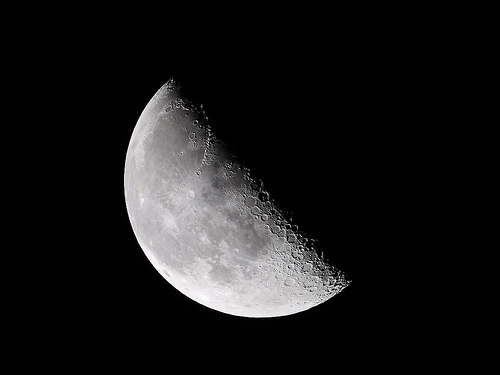
\includegraphics[width=65mm]{img/moon.jpg}
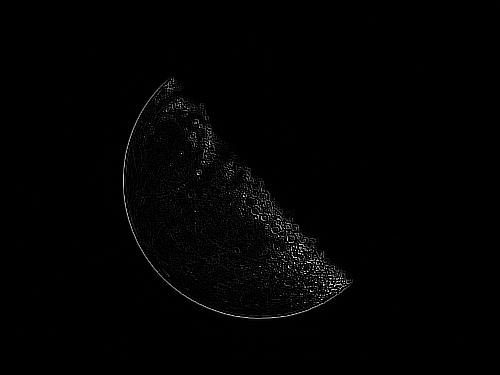
\includegraphics[width=65mm]{img/moonLap.jpg}
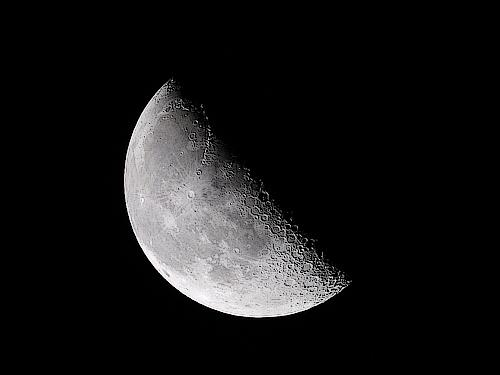
\includegraphics[width=65mm]{img/moonEn.jpg}
\caption{1)slika 2)laplacian 3)poboljšana slika dodavanjem laplacian-a}
\label{overflow}
\end{figure}

Ova operacija može da se implementira u jednom prolazu tako što će da se modifikuje kernel. Operacija koja je izvršena na predhodonj slici može da se predstavi ovako:

\begin{center}
$g(x, y) = f(x, y) - \Delta^{2}f(x, y) = 5f(x, y) - [f(x + 1, y) + f(x - 1, y) + f(x, y - 1) + f(x, y + 1)]$.\\
\end{center} 

Na osnovu ove funkcije možemo da zaključimo da će kernel da izlgeda ovako:

\[
\begin{bmatrix}
     0 & -1 & 0 \\
     -1 & 5 & -1 \\
     0 & -1 & 0 \\
\end{bmatrix}
\begin{bmatrix}
     -1 & -1 & -1 \\
     -1 & 9 & -1 \\
     -1 & -1 & -1 \\
\end{bmatrix}
\]. 

Postoji još jedan način za postizanje poboljšanja slike. Naime ivice slike mogu da se odrede tako što će od ogriginalne slike oduzeti slika nad kojom je primenjen smoothing filter. Pošto smoothing filter ima suprotno dejstvo od shaprening filtera oduzimanje će dati isti rezultat kao primena sharpening filtera. 

Kao što je rečeno ranije za filtriranje slike može da se koristi i prvi izvod. Prvi izvod se za filtriranje koristi tako što se računa dužina gradijenata po x i y osi. Za funkciju $f(x, y)$ gradijent u koordinatama $(x, y)$ se definiše kao vektor: \\

\[
\Delta \textbf{f}
=
\begin{bmatrix}
     G_{x} \\
     G_{y} \\
\end{bmatrix}
=
\begin{bmatrix}
     \dfrac{\delta f}{\delta x} \\
     \\
     \dfrac{\delta f}{\delta y} \\
\end{bmatrix}
\]. 

Dužina vektora se računa kao: 

\begin{center}
	$\Delta \emph{f} = mag(\Delta \textbf{f}) = [G_{x}^{2} + [G_{y}^{2}]^{1/2} = [ (\dfrac{\delta f}{\delta x})^{2} +  (\dfrac{\delta f}{\delta y})^{2} ]^{1/2}$. \\
\end{center}

Gradijenti su linearne funkcije, ali njihova funkcija dužine nije jer sadrži stepene operacije. Sa druge strane gradijenti nisu invarijantni u odnosu na rotaciju dok funkcija njihove dužine jeste, pa se zbog toga ona koristi. Iako nije tačno dužina vektora gradijenta se često naziva gradijent. Pošto nije lako primeniti ovu funkciju nad slikom koja ima diskretne vrednosti za potrebe obrade slike se obično koristi aproksimacija dužine gradijenta $\Delta \approx |G_{x}| + |G_{y}|$. Ova funkcija je lakša za izračunavanje i prepoznaje promene, ali generalno gubi osobinu invarijacije u odnosu na rotaciju. Kao što je slučaj kod laplacian-a izotropska osobina očuvana je zahvaljujući odabiru maske i dodavanju dijagonalnih elemenata. 

Ako je region na slici za kernel veličine 3 x 3 definisan kao

 \[
\begin{bmatrix}
     z_{1} & z_{2} & z_{3} \\
     z_{4} & z_{5} & z_{6} \\
     z_{7} & z_{8} & z_{9} \\
\end{bmatrix}
\].

gde $z_{5}$ predstavlja $f(x, y)$, a $z_{1}$ predstavlja $f(x - 1, y - 1)$ onda je $G_{x} = (z_{9} - z_{5})$ i $G_{y} = (z_{8} - z_{6})$. Ovo je prva predložena definicija za računanje prvih izvoda. Sledi da je gradijent:

\begin{center}
$\Delta \emph{f} \approx |z_{9} - z_{5}| + |z_{8} - z_{6}|.$\\
\end{center}

Kernel za ovako definisan gradient se naziva Robertsov kros-gradijent operator i izgleda ovako:\\

 \[
\begin{bmatrix}
     -1 & 0 \\
     0 & 1 \\
\end{bmatrix}
\begin{bmatrix}
     0 & -1 \\
     1 & 0 \\
\end{bmatrix}
\].

Pošto za kernele nije uobičajno da imaju parne dimenzije uvodi se ovakva definicija gradijenta. Ako imamo kernel veličine $3 x 3$ funkcija gradijenta izgleda ovako: 

\begin{center}
$\Delta \emph{f} \approx |(z_7 + 2z_8 + z_9) - (z_1 + 2z_2 + z_3)| + |(z_3 + 2z_6 + z_9) - (z_1 + 2z_4 + z_7)|$.\\
\end{center}

Kerneli za ovu funkciju izgledaju ovako: \\

 \[
\begin{bmatrix}
     -1 & -2 & -1 \\
     0 & 0 & 0 \\
     1 & 2 & 1 \\
\end{bmatrix}
\begin{bmatrix}
     -1 & 0 & 1 \\
     -2 & 0 & 2 \\
     -1 & 0 & 1 \\
\end{bmatrix}
\].

Ovi kerneli su poznatiji kao Sobelovi operatori. 

\begin{figure}[ht!]
\centering
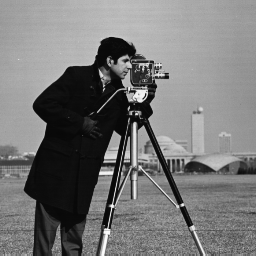
\includegraphics[width=60mm]{img/img.png}

\includegraphics[width=60mm]{img/imgSob.png}
\caption{1)slika 2)sobel}
\label{overflow}
\end{figure}

\subsection{Kombinovanje filtara}%%%%%%%%%%%%%%%%%%%%%%%

Predhodno prikazani filtri za uklanjanje šuma i određivanje ivica imaju veliku primenu u obradi slike. U većini slučaja oni se koriste kao deo nekog većeg procesa. U predhodnim poglavljima je navedeno nekoliko slučajeva. Smoothing filtri se koriste da bi se uklonili objekti koji nisu od važnosti za ekstrakciju objekata sa slike. Takođe ovi filtri mogu da se koriste za određivanje ivica i poboljšanje slike, tako što će se na sliku dodati detalji dobijeni oduzimanjem slike i njene zamućene verzije, koja se dobija primenom smoothing filtra. Detalji dobijeni primenom filtara za određivanje ivica i detalja mogu da se dodaju na sliku i cilju poboljšanja i naglašavanja detalja. 

Jasno je da se ovi filtri koriste u kombinaciji sa drugim filtrima i kao deo nekog većeg procesa. Oni mogu međusobno da se kombinuju. Postoje i složeni filtri koji su napravlejni koristeći koncepte ova dva tipa filtara. To je nejmoćniji tip filtara koji kao rezultat daje slike kod kojih se uklanja šum, što je odlika smoothing filtara, ali se pri tome slika ne zamućuje, čuvaju se ivice, što je odlika sharpening filtara. Dva najpoznatija ovakva filtra su \emph{Bilateral filter} i \emph{Guided filter} kojim se ovaj rad detaljnije bavi u nastavku.  

\section{Guided filter}%%%%%%%%%%%%%%%%%%%%%%%%

\subsection{Uvod}%%%%%%%%%%%%%%%%%%%%%%%

Veliki broj aplikacija u oblastima kompjuterske vizije i računarske grafike sadrže proces zadužen za filtriranje slika, u cilju uklanjanja i/ili izvlačenja podataka sa slike. Linearni filtri invarijantni na tranziciju, kao što su mean, Laplacinan, Gausov i Sobelovi filtri, se široko koriste prilikom obrade slike, za restauraciju, zamućivanje i izoštravanje, detekciju ivica, izvlačenje podataka, dinamičku kompresiju itd. Ovi filteri su prostorno invarijantni i nezavisni od sadržaja slike. 

Pa ipak oni nekad nemogu da zadovolje očekivani odgovor neke obrade. Zbog toga se ovde uvodi pojam slike vodiča \emph{(eng. guide)}, koja sadrži dodatne inforamcije koje mogu da se ikoriste pri filtriranju i poboljšaju rezultat. Ovaj koncept je prvi put upotrebljen u procesu difuzije \emph{(eng. anisotropic diffusion)}, u kojem gradijenti filtrirane slike služe kao vodič za ovaj proces i tako ovaj proces izbegava da uništi oštrinu ivica. Takođe WLS filter \emph{(eng. weighted least squares)} koristi ulaznu sliku kao vodič, optimizuje kvadratnu funkciju, koja je ekvivalentna procesu difuzije, koji je malopre pomenut. U mnogim primenama kao slika vodič može da se koristi različita slika u odnosu na onu koja se filtrira. Npr. kod procesa uklanjanja magle sa slike, kao slika vodič se koristi procena količine smetnji na slici, koja treba da se filtrira. Većina ovih procesa je implementirana, optimizacijom kvaratne funkcije, čiji su parametri uzeti iz slike vodiča. Rešenje je predstavljeno rešenjem velikih retko popunjenih matrica. Ovakve nehomogene matrice predstvaljaju filtere koji su invarijantni u odnosu na tranziciju. Iako su ovakvi filtri efikasni, oni mogu da budu zahtevni za izvršavanje.

Drugi način da se iskoristi slika vodič je da se njene osobine eksplicitno iskažu u kernelu. \emph{Bilateral filter} je najpoznatiji primer takvog filtera. Rezultat koji piksel dobija, kod ovog filtriranja, je težinska prosečna vrednost piksela i njegovih suseda, gde težine zavise od sličnosti piksela u voidč slici. Vodič slika moće i sama da bude ulazna slika u ovom filtru. \emph{Bilateral filter} može da izglača siten fluktuacije, a da pri tome zadrži ivice. Problem ovog filtra je što ima loše artifakte koji se javljaju blizu ivica. Dolazi do promene boje blizu ivica. Takođe problem je implementirati efikasan algoritam, metodi koji ubrzavaju ovaj algoritam sa druge strane utiču na preciznost njegove obrade.

U radovima [3] i [4] se predlaže \emph{Guided filter} ili vođeni filter. Rezultat filtriranja je lokalna linearna transformacija slike vodiča. Sa jedne strane ovaj filter ima dobre osobine, pošto čuva ivice slike, a sa druge strane nema loše artifakte kao \emph{Bilateral filter}. \emph{Guided filter} može da se koristi kao smoothing filter, ali njegova namena prevazilazi samo to. Uz pomoć slike vodiča rezultat ovog filtriranja će biti slika koja je manje zamućena od originalne slike i bolje struktuirana od nje. Ovaj filter se pokazao dobro u raznim primenama kao što su poboljšanje slike, ukljanjanje šuma, HDR kompresija, mating idt. Još jedan prednost \emph{Guided filter}-a je to što ima složenost $O(n)$, gde je $n$ broj piksela slike. Moće da se koristi kako na jednokanalnim slikama tako i na višekanalnim slikama. Prema radovima [3] i [4] ovo je najbrži filter ove namene, koji na CPU implementaciji obrađuje 1 mega piksel(1024 x 1024) za 40ms. 

\subsection{Slične ideje}%%%%%%%%%%%%%%%%%%%%%%%  

\emph{Bilateral filter} je tipičan primer ovog tipa filtara i jedan od prvih koji je zamišljen. To su filtri koji služe za smoothing ali pri tome zadržavaju ivice slike. Rezultat filtriranja svakog piksela slike je težinska srednja vrednost piksela i njegovih suseda. Ima široku primenu. Koristi se za redukciju šuma, HDR kompresiju, dekompoziciju detalja. Generalizovan je u implementaciji \emph{joint bilateral filter}-a, gde se težine računaju u odnosu na sliku vodiča, za koju se koristi posebna slika. Ovaj filter se koristi kada se od filtriranja ne očekuje da pruži inforamcije o ivicama, npr. kada slika ima dosta šuma ili kada je rezultat koji treba dalje da se iskoristi. Iako je \emph{Bilateral filter} veoma popularan i intuitivan za shvatanje, on ima limitacije. 

Predhodno spomenuti loši artifakti koji se javljaju blizu ivica, jer je gausova funkcija nestabilna blizu ivica zbog velikih razlika u vrednostima piksela. Drugi problem se odnosi na složenost algoritma. Brute-force implementacija ima složenost $O(Nr^2)$, gde je $N$ broj piksela na slici, a $r$ je radius kernela (dimenzija kernela je $a = 2r + 1$). Jasno je da složenost zavisi od veličine kernela što može da bude loše ako se koriste veliki kerneli. Postoje rešenja koja koriste razne metode kao što su distribuirani histogrami koji složenost smanjuju na $O(n \log{r})$. Postoji i metod za redukciju složenosti na $O(n)$ korišćenjem integralnih histograma (kao lookup tabela). Međutim konstrukcija histograma je primena filtera u prostornom domenu, pa možemo da zaključimo da ovaj proces zahteba dodatne korake. Postoji još jedan pristup čija je složenost $O(n)$, a koji se oslanja na agresivno smanjenje slike \emph{subsampling}, čime se gube detalji. Važno je naglasiti da sva spomenuta rešenja koja imaju lineranu složenost, sa druge strane utiču na degradaciju preciznosti. Pošto \emph{Bilateral filter} ima svoje limitacije ljudi su krenuli da istražuju nove metode za filtre koji uglačavaju sliku, a pri tome čuvaju ivice. 

Nasuprot lineranim filterima postoje implicitni filteri koji se dobijaju optimizacijom funkcije greške i rešavanjem linearnog sistema jednačina, što je ekvivalentno implicitnom filtriranju slike korišćenjem inverzne matrice. Ovi filtri takođe imaju široku primenu u segmentaciji slike, kolorizaciji slike, itd. Iako su ovakvi filtri efikasni i daju kvalitetan rezultat, međutim računanje linearnih sistema može da bude veoma složeno. Direktna rešenja kao što je gausova eliminacija, nisu praktični, zbog velkog zauzeća memorije. Iterativna rešenja sporo konvergiraju. Uočeno je da su implicitni filteri slični kao eksplicitni. 

Očuvanje ivica može da se postigne i filterima koji ne koriste srednje vrednosti susednih piksela. Najpoznatiji je median filter koji je objašnjen u poglavlju 2.2.           

\subsection{Definicija filtra}%%%%%%%%%%%%%%%%%%%%%%%

Prvo ćemo definisati uopšteni proces linearnog invariantnog filtriranja, koji koristi sliku vodič $I$, sliku koja se filtrira $p$ i sliku koja je rezultat filtriranja $q$. $I$ i $p$ su zadati na početku procesa i oni mogu da budu identični. Rezultat filtriranja piksela $i$ će biti: 

\begin{center}
	$q_i = \sum_{j} W_{ij}(I)p_j$,
\end{center}

gde su $i$ i $j$ indeksi piksela, kernel filtera $W_{ij}$ je funkcija slike vodiča $I$ i nezavisna je od $p$. Ovaj filter je linearan u odnosu na $p$. 

Sada ćemo definisati guided filter. Predpostavka je da je guided filter loklano linearan model između slike vodiča $I$ i rezultata filtriranja $q$. Za $q$ predpostavljamo da je linearna transforamcija slike $I$ u prozoru $w_k$ centriranom u pikselu $k$:

\begin{center}
	$q_i = a_kI_i + b_k, \forall \epsilon w_k$,
\end{center}

gde su $(a_k, b_k)$ linearni koeficijenti za koje ćemo predpostaviti da su konstantni u $w_k$. Za $w_k$ koristimo kvadratni prozor radiusa $r$. Ovaj lokalni linearni model garantuje da će $q$ imati ivicu samo ako $I$ ima tu istu ivicu, jer je $\Delta q = a\Delta I$. Da bi odredili linearne koeficijente $(a_k, b_k)$, trebaju nam ograničenja slike koja se filtrira $p$. Rezultat filtriranja određeog piksela $q_i$ se dobija tako što se od $p_i$ oduzimaju neke neželjene komponente kao što su razni detalji i šum: $q_i = p_i - n_i$. Mi tražimo rešenje koje će minimizovati razliku između $p$ i $q$, pod sulovom da je ta funkcija linearna. Konkretno za svaki prozor $w_k$ treba da minimizujemo sledeću funkciju greške:

\begin{center}
	$E(a_k, b_k) = \sum_{i \epsilon w_k} ((a_kI_i + b_k - p_i)^2 + \varepsilon a_k^2)$.
\end{center}

$\varepsilon$ je regularizacioni parametar koji služi da smanji uticaj $a_k$, ako je njena vrednost velika. Minimizacija ove jednačine predstavlja problem koji se rešava linearnom regresijom. Ovde ne ulazimo u detalje ovog rešenja već dajemo rešenja direktno:

\begin{center}
	$a_k = \dfrac{\dfrac{1}{|w|} \sum_{i \epsilon w_k} I_ip_i - \mu_k \overline{p_k}}{\sigma_k^2 + \varepsilon}$,
\end{center}

\begin{center}
	$b_k = \overline{p_k} - a_k \mu_k$.
\end{center}

$\mu_k$ i $\sigma_k^2$ su srednja vrednost i varijansa piksela slike $I$ u prozoru $w_k$, a $|w|$ je broj piksela u $w_k$, $\overline{p_k} = \dfrac{1}{|w|} \sum_{i \epsilon w_k} p_i$ je srednja vrednost piksela slike u $w_k$. Kada smo sračunali linearne koeficijente $(a_k, b_k)$, možemo da nastavimo sa postupkom za izračunavanje rezultata $q_i$. Pošto je će piksel $i$ biti deo različitih prozora $w_k$, prilikom filtriranja, ne možemo da koristimo jedinstvene koeficijente $(a_k, b_k)$ za jedan piksel. Zbog toga ćemo u obzir uzeti sve moguće vrednosti koeficijenata za $q_i$. Kada izračunamo vrednosti $(a_k, b_k)$ za svaki piksel ulazne slike, rezultat filtriranja će biti:

\begin{center}
	$q_i = \dfrac{1}{|w|} \sum_{k|i \epsilon w_k} (a_kI_i + b_k)$.
\end{center}    

Pošto su prozori $w_k$ kvadratnog oblika i simetrični su, možemo da primetimo da je $\sum_{k|i \epsilon w_k} a_k = \sum_{k \epsilon w_i} a_k$, pa formula može da se napiše ovako:

\begin{center}
	$q_i = \overline{a_i}I_i + \overline{b_i}$,
\end{center}

gde su $\overline{a_i} = \dfrac{1}{|w|}\sum_{k \epsilon w_i} a_k$ i $\overline{b_i} = \dfrac{1}{|w|}\sum_{k \epsilon w_i} b_k$ srednje vrednosti iz svih prozora u kojima je $q_i$ sadržan. Sa promenom koja je uvedena u ovoj jednačini gubimo sličnost između $\Delta q$ i $\Delta I$ na mestima gde su ivice, jer linearni koeficijenti $(\overline{a_i}, \overline{b_i})$ variraju u zavisnosti od prostora. Međutim pošto su oni rezultat filtra srednje vrednosti, možemo da očekujemo da će njihovi graijenti biti mnogo manji nego gradijenti $I$ blizu jakih ivica. U ovoj situaciji možemo da kažemo da je $\Delta q \approx \overline{a} \Delta I$, što znači da će nagle promene intenziteta na $I$ biti sačuvane i na $q$. 

U nastavku je dat pseudo kod algoritma, koji je definisan na osonvu predhodinh jednačina. $f_{mean}$ je filter srednje vrednosti sa radiusom $r$. \emph{corr, var i cov} označavaju redom korelaciju, varijansu i kovarijansu. 

\textbf{Algoritam Guided filter}\\

\textbf{Ulaz:} slika koja se filtrira $p$, slika vodič $I$, radius $r$, parametar regularizacije $\varepsilon$.\\

\textbf{Izlaz:} filtrirana slika $q$.\\

1: $mean_I = f_{mean}(I)$

\hspace{4mm} $mean_p = f_{mean}(p)$

\hspace{4mm} $corr_I = f_{mean}(I .* I)$

\hspace{4mm} $corr_{Ip} = f_{mean}(I .* p)$

2: $var_I = corr_I - mean_I .* mean_I$

\hspace{4mm}  $cov_{Ip} = corr_{Ip} - mean_I .* mean_p$

3: $a = cov_{Ip} ./ (var_I + \varepsilon)$

\hspace{4mm} $b = mean_p - a .*  mean_I$

4: $mean_a = f_{mean}(a)$

\hspace{4mm} $mean_b = f_{mean}(b)$

5: $q = mean_a .* I + mean_b$

$ .*  i  ./ $ su podkompoentno množenje i deljenje matrica.


\subsection{Očuvanje ivica}%%%%%%%%%%%%%%%%%%%%%%%

S obzirom da je jedan od glavnih prednosti ovog filtra očuvanje ivica, ovde ćemo proveriti tu osobinu. Na sledećoj slici su prikazani primeri filtriranja guided filtrom, korišćenjem različitih parametara. Ovo je primer gde se koristi identična slika i kao ulaz i kao slika vodič. Na ovom primeru možemo da vidimo da se guided filter ponaša kao filter koji čuva ivice, iako je njegova namena da uglača sliku. 
Na primerima koji su prikazani na slici 13 možemo da uočimo ove osobine i možemo da primetimo razliku između guided filtra i filtara prikazanih u poglavlju 2.2 koji tađe služe za uglačavanje slike.

\begin{figure}[ht!]
\centering
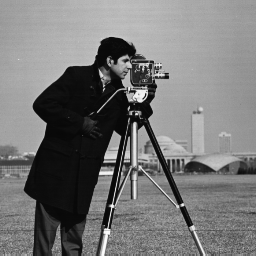
\includegraphics[width=60mm]{img/img.png}
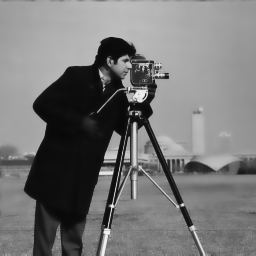
\includegraphics[width=60mm]{img/imgGF2_01.png}
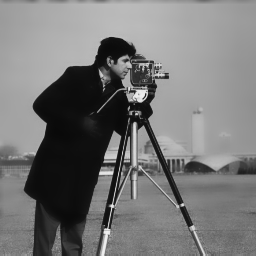
\includegraphics[width=60mm]{img/imgGF4_01.png}
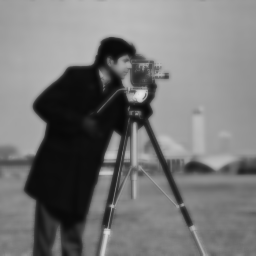
\includegraphics[width=60mm]{img/imgGF2_16.png}
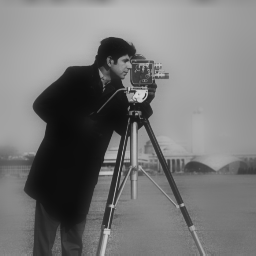
\includegraphics[width=60mm]{img/imgGF8_04.png}
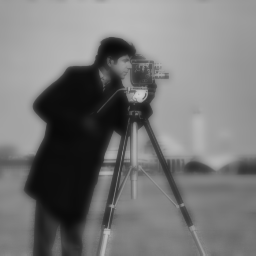
\includegraphics[width=60mm]{img/imgGF4_16.png}
\caption{1)slika; slika filtrirana guided filtrom sa parametrima 2) $r = 2 \varepsilon = 0.01$; 3) $r = 4 \varepsilon = 0.01$; 2) $r = 2 \varepsilon = 0.16$; 2) $r = 8 \varepsilon = 0.04$; 2) $r = 4 \varepsilon = 0.16$}
\label{overflow}
\end{figure}

Sa slike 13 možemo da zaključimo da regularizacioni parametar $\varepsilon$ utiče na to koliko će slika biti zamućena odnosno šta je na slici ivica koja trba da se sačuva, a radius prozora $r$ utiče na to koliko će suseda biti korišćeno pri filtriranju, što će kao kod smoothing filtara uticati na količinu uklonjenog šuma. 

Osobina očuvanja ivice može intuitivno da se objasni ovako, ako uzmemo da je $I \equiv p$. U ovom slučaju će $a_k$ i $b_k$ koji su definisani u predhodnom poglavlju da izgledaju ovako $a_k = \sigma_k^2 / (\sigma_k^2 + \varepsilon)$, $b_k = (1 - a_k)\mu_k$. Jasno je da kada je $\varepsilon = 0$ onda je $a_k = 1$ i $b_k = 0$, pa će $q = I$. Kada je $\varepsilon > 0$ onda treba da razmotrimo dva slučaja. Prvi je slučaj ''visoke varijanse'', kada $I$ ima dosta promena vrednosti unutar prozora $w_k$, tada je $\sigma_k^2 >> \varepsilon$, pa je $a_k \approx 1$ i $b_k \approx 0$. Drugi je slučaj ''ravnog područija'', kada $I$ ima skoro identične vrednosti u prozoru $w_k$, tada je $a_k \approx 0$ i $b_k \approx \mu_k$. 

Kada računamo srednje vrednosti za $a_k$ i $b_k$ da bi dobili $\overline{a_i}$ i $\overline{b_i}$, koje koristimo da bi dobili rezultat (kao što je definisano u predhodom poglavlju), tada će, ako se piksel nalazi u prozoru ''visoke varijanse'', njegova vrednost biti nepromenjena ($a \approx 1, b \approx 0, q \approx p$). U slučaju da se piksel nalazi u oblasti ''ravnog područija'', tada će rezultujuća vredost biti srednja vrednost piksela suseda ($a \approx 0, b \approx \mu, q \approx \overline{\mu}$). Ova dva slučaja su određena parametrom $\varepsilon$. Delovi slike, gde je varijansa $\sigma^2$ mnogo manja od $\varepsilon$, su uglačana odnosno smooth-ovana, a mesta gde je $\sigma^2$ mnogo veća od $\varepsilon$ su očuvana. U suštini parametar regularizacije $\varepsilon$ određuje šta je ivica, odnosno šta treba da ostane nepromenjeno.   

\subsection{Osobine filtra}%%%%%%%%%%%%%%%%%%%%%%%      

\subsection{Izračunavanje i efikasnost}%%%%%%%%%%%%%%%%%%%%%%% 

Glavna prednost guided filtra u odnosu na slične filtre kao što je bilateral filter, koji je spomenut u poglavlju 3.2, se ogleda u tome što ima složenost $O(n)$. Njegova složenost je nezavisna od radiusa prozora (kernel) koji se koristi za filtriranje i od intenziteta fitriranja. Kod bilateral filtra složenost, kao što je pokazano u poglavlju 3.2, zavisi od veličine prozora. Umesto da direktne primene konvolucije, kao kod većine konvolucionih filtara, ovde se vrednost rezultujućeg piksela računa kao linearna funkcija definisana u 3.3. Prvo se računaju koeficijenti $a_k$ i $b_k$.

\begin{center}
	$a_k = \dfrac{\dfrac{1}{|w|} \sum_{i \epsilon w_k} I_ip_i - \mu_k \overline{p_k}}{\sigma_k^2 + \varepsilon}$,
\end{center}

\begin{center}
	$b_k = \overline{p_k} - a_k \mu_k$.
\end{center}

Ovde možemo da primetimo da postoji nekoliko sumiranja:  $\sum_{i \epsilon w_k} I_ip_i, \mu_k$ je srednja vrednost, $\sigma_k^2$ je varijansa, $\overline{p_k}$ srednja vrednost piksela. Srednja vrednost i varijnsa takođe zahtevaju izračunavanje sume ogovarajućih piksela. Ove sume možemo da izračunamo u $O(1)$ korišćenjem \emph{look-up} tabela takozvanih integralnih slika. Kada se izračunaju koeficijenti $a_k$ i $b_k$, onda se rezultat dobija kao:

 \begin{center}
	$q_i = \overline{a_i}I_i + \overline{b_i}$,
\end{center}

gde su $\overline{a_i} = \dfrac{1}{|w|}\sum_{k \epsilon w_i} a_k$ i $\overline{b_i} = \dfrac{1}{|w|}\sum_{k \epsilon w_i} b_k$ srednje vrednosti iz svih prozora u kojima je $q_i$ sadržan. Ove dve sume takođe možemo da izračunamo u $O(1)$ korišćenjem  integralnih slika. Pošto je složenost računanja vrednosti za jedna piksel $O(1)$ možemo da zaključimo da  će složenost algoritma biti $O(n)$, gde je $n$ broj piksela.

Integralna slika je

\subsection{Poboljšanje}%%%%%%%%%%%%%%%%%%%%%%%   

\subsection{Eksperimenti}%%%%%%%%%%%%%%%%%%%%%%%

 

\section{Primena}%%%%%%%%%%%%%%%%%%%%%%%%%%

\newpage
\addcontentsline{toc}{section}{Literatura}
\begin{thebibliography}{10}

\bibitem{ComputerGraphic}
\emph{\href{http://www.graphics.cornell.edu/online/tutorial/}{What is Computer Graphics?}},
Cornell University Program of Computer Graphics,
1998.

\bibitem{DigitalImageProcessing}
Rafael C. Gonzalez, Richard E. Woods,
\emph{\href{https://books.google.rs/books?id=8uGOnjRGEzoC&redir_esc=y}{Digital Image Processing}},
Prentice Hall,
2008.

\bibitem{GuidedFilter1}
Kaiming He, Jian Sun, Xiaoou Tang,
\emph{\href{http://kaiminghe.com/publications/eccv10guidedfilter.pdf}{Guided Image Filtering}},
ECCV,
2010.

\bibitem{GuidedFilter2}
Kaiming He, Jian Sun, Xiaoou Tang,
\emph{\href{http://kaiminghe.com/publications/pami12guidedfilter.pdf}{Guided Image Filtering}},
TPAMI,
2013.

\bibitem{GuidedFilter3}
Kaiming He, Jian Sun
\emph{\href{https://arxiv.org/pdf/1505.00996.pdf}{Fast Guided Filter}},
arXiv,
2015.

\end{thebibliography}

\end{document}